One of the aims of the project was to test the vehicle in a controlled environment to acquire data and assess the vehicle’s performance. This would allow for further developments on the vehicle but also further the understanding of the concept and what it takes to build a downwind faster than the wind vehicle. With the prototype being too large to be tested on a treadmill as had been done previously by Rick Cavallaro in \cite{rick2008youtube}, the best option for testing the vehicle in a quantifiable way was to use the rolling road in the R.J. Mitchell Wind tunnel at the University of Southampton. Before testing, the main quantities for which data was to be acquired were outlined. Included, were the drivetrain efficiency, vehicle drag and overall performance. The completed tests ran the vehicle on the rolling road in the wind tunnel with wheel arm mounts holding the vehicle in place. Aerodynamic drag values for the vehicle were obtained in both directions.

\subsection{Inputs} 

For the wind tunnel test, there were four main inputs for each experimental test: the rolling road speed, wind speed, propeller blade pitch and the gear ratio. It was initially intended to have an interchangeable gear ratio. However, the sprockets were made from hardened steel, so the gear ratio had to be fixed because threading these components was not feasible with the available means. A 1:1 chain gear ratio was chosen as this outputted the right RPM for the propeller given the wheel size. The chain sprockets were then welded to the gearbox shaft. The rolling road speed was varied for each test case, starting at low speeds and increasing in increments of $0.5\mathbf{m/s}$ or $1\mathbf{m/s}$ to ensure that a wide range of testing cases were available for analysis. Modulating the pitch of the propeller would help in finding an optimal setup to maximise performance, hence furthering the understanding of the characteristics of the DWFTTW prototype. The vehicle was monitored at all points during testing to ensure normal operation and avoid catastrophic failures.

\begin{figure}[!htbp]
    \centering
    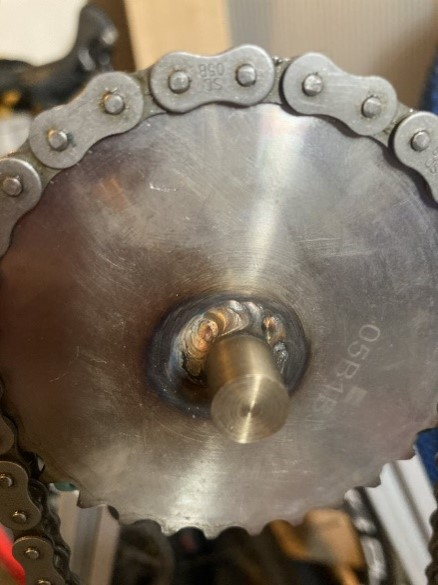
\includegraphics{images/part10/chaincog.jpg}
    \caption{Sprocket welded to propeller shaft}
    \label{fig:weldedsprocket}
\end{figure}

\subsection{Wind tunnel testing plan}

A test session of three consecutive days was initially intended in the R.J. Mitchell wind tunnel. This would ensure the completion of all the planned tests while sparing the time required for setting experiments up. From analysis, three main test conditions, to simulate a normal vehicle operational environment, were outlined. The cases are looking at the vehicle under slower than, the same speed as, and faster than the wind regime.

\begin{figure}[!htbp]
    \centering
    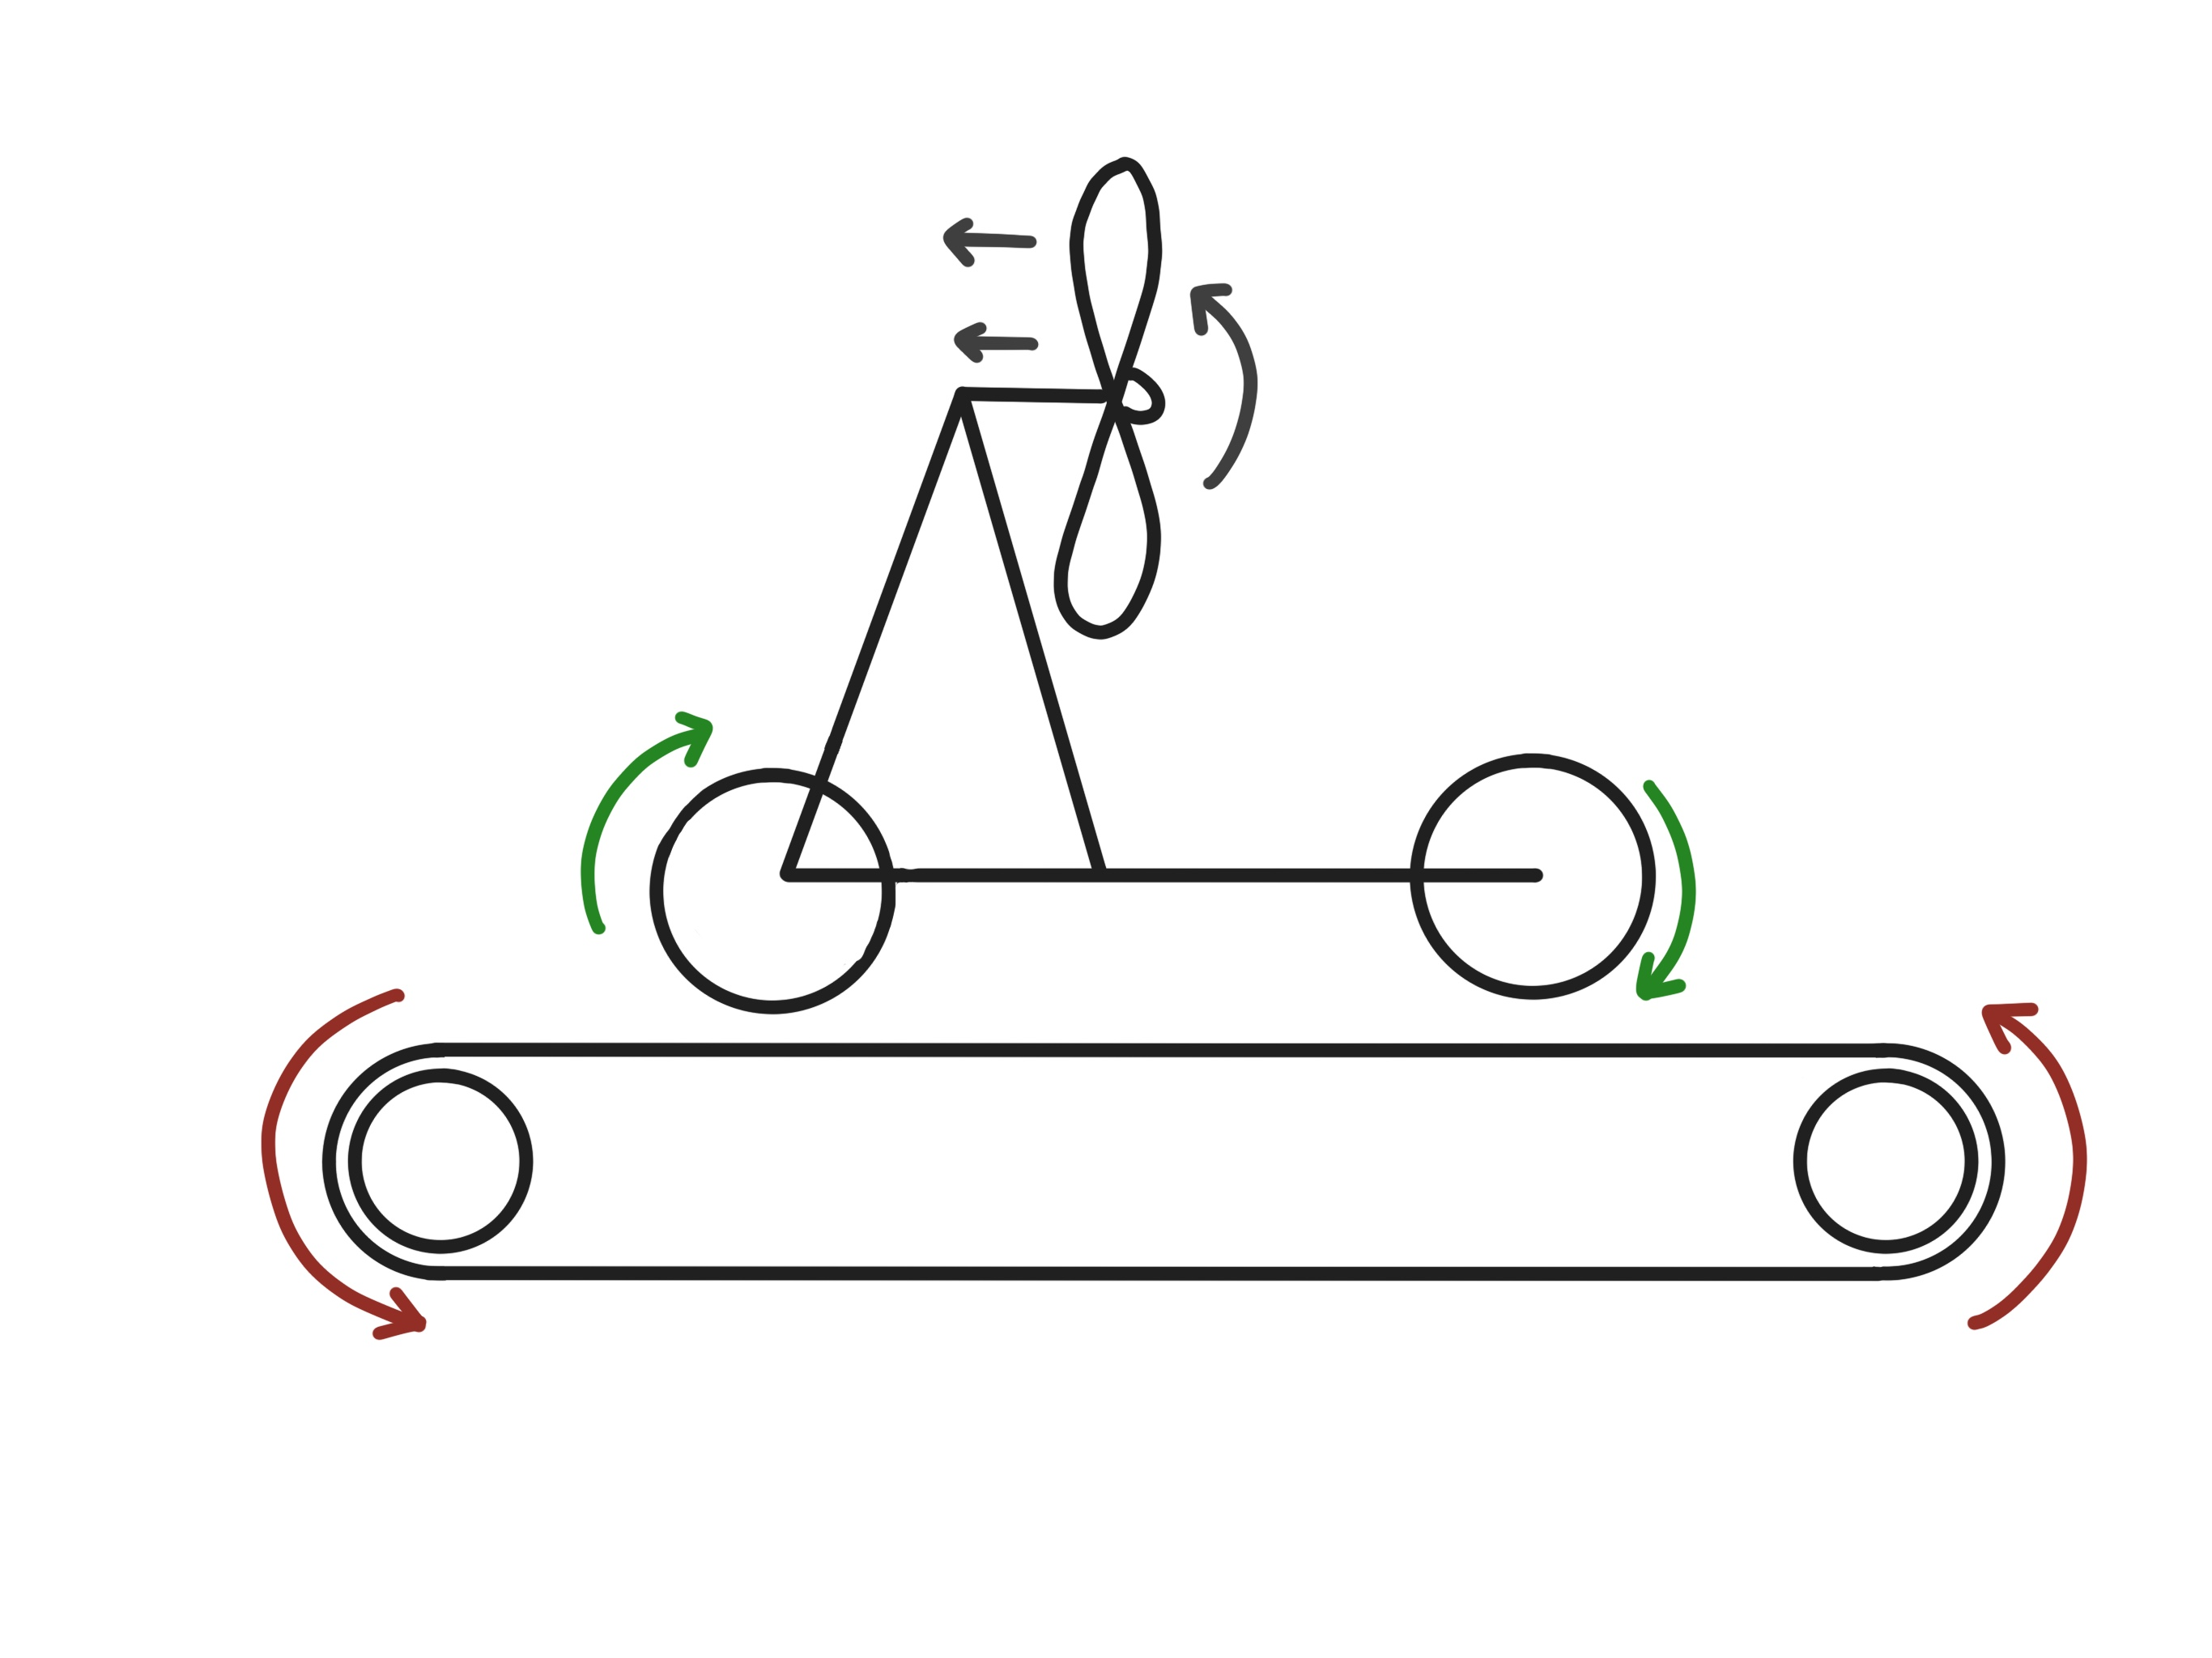
\includegraphics[width=0.4\linewidth]{images/part10/expebaseline.jpg}
    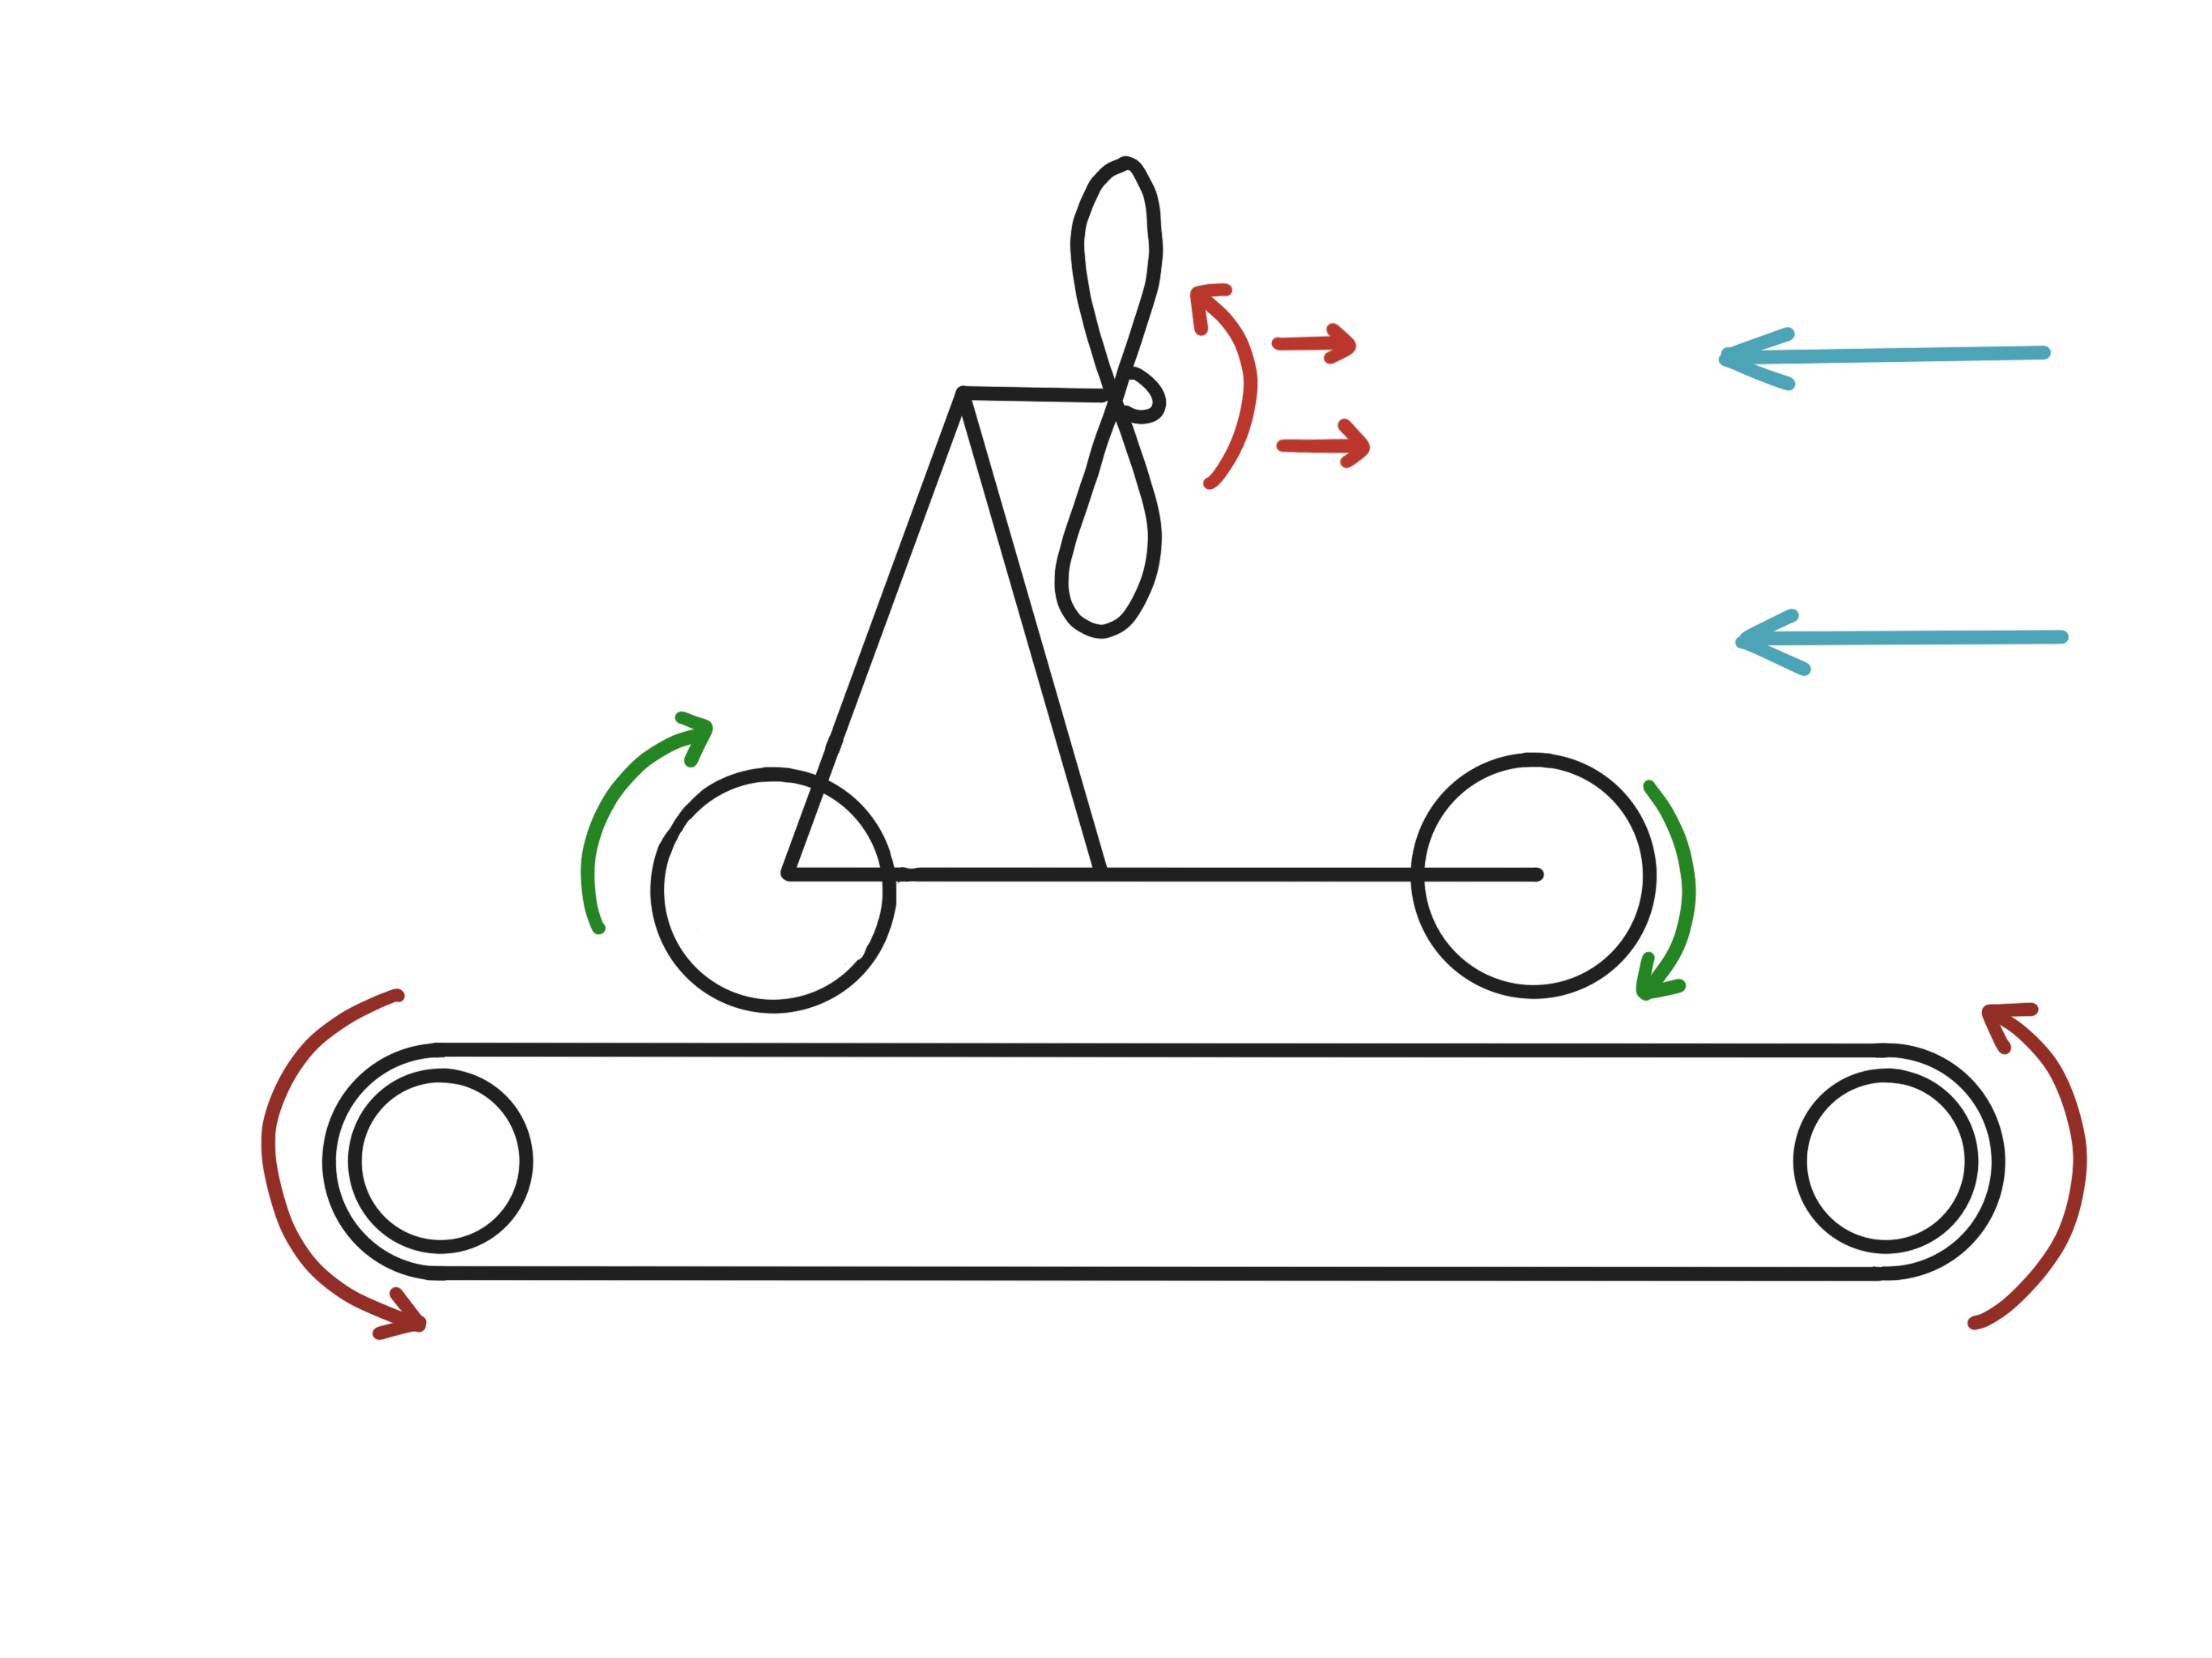
\includegraphics[width=0.4\linewidth]{images/part10/fasterthanwind.jpg}
    \caption{"Baseline" experimental setup (left) and "faster than wind" experimental setup (right).}
    \label{fig:baseline}
\end{figure}

With the aim being to determine the maximum speed the vehicle was able to reach, several experimental setups were defined. The case in which the ground speed is equal to the wind speed was the simplest scenario to recreate as is illustrated in the baseline diagram in Figure \ref{fig:baseline} (left). It required the rolling road to be moving along with the vehicle mounted on top. This test was run to determine which drag or thrust was produced while the vehicle was moving at wind speed. Based on the outcome, various testing setups were defined to simulate the relevant operating conditions. This setup will be referred to as the baseline setup for added clarity. For faster than the wind operation Figure \ref{fig:baseline} (right), the wind tunnel was to be used in combination with the rolling road to simulate on-coming wind.

Due to the rolling road only being capable of operating in the same direction as the wind flow, reproducing slower than wind operation was less direct. To achieve it, one of the considered options was to rotate the vehicle in the wind tunnel test section while inverting the gearbox to run the drivetrain in reverse. This made it possible for the prototype to run with the wind differential pushing it, yielding insight into how this would affect performance. However, this option was not carried out as it would have meant additional precious time being spent setting up. It also introduced the requirement to reconfigure to the gearbox, which was meant to be welded. The other option for this case was to run the baseline setup and quantify the rolling resistance. In turn, from this and the before-hand quantified drag, the equilibrium point could be determined analytically by summing the various forces.

\subsection{Project timings}

The initial wind tunnel testing plan was a three-day testing period in which all the measurements and analysis would be completed as well as some further testing for the visual experiments. Time management proved crucial for this project as planning the wind tunnel days had to be done well in advance. Therefore, early contact was made with the wind tunnel team, so that the tests could be designed and organised as early as possible. Regular meetings were arranged to facilitate progress and impose strict deadlines for manufacturing and design.

Despite this, due to manufacturing issues, the propeller was not ready before the planned three-day testing period. Some experiments could be carried out by disregarding the propeller, but complete vehicle testing was not possible. Hence the test sessions were split into two sets: a one day session to test the drivetrain, then a two days session to test the full vehicle operation. This meant that a first test could be carried out without the propeller, but also conveniently sparing time for the EDMC to finish the missing parts. It also became possible to spot potential issues with the structure of the vehicle early thanks to the first test and have enough time before the next wind tunnel session to correct them. The first test day was conducted in mid-February while the second was completed in March.
 

\subsection{Load measurement using the rolling road}

The best way of quantifying the loss contribution of each element of the vehicle was to use the wind tunnel’s rolling road and measure the increased drag force on the system induced when adding each component to the vehicle. By running the rolling road at a set range of velocities, measurements of the force applied to the vehicle could be taken using the load cells mounted on each side. The force required to overcome each element of the vehicle added gradually was plotted, and the losses induced by each component was quantified.

The data collected for this experiment was comprehensive and covered all the main drivetrain components meaning an in-depth analysis of the limiting factors of the vehicle could be completed. Although this experiment quantified the loss contributions of many components of the prototype, no way could be found, given the available installations, to evaluate the efficiency of the propeller shaft bearings. Therefore it was not possible to dissociate the contributions of the chain and the top bearings to the losses without speculating or making further assumptions that were out of the scope of this project.


\subsection{Load cell and force measurements}

The load cell was the main point of connection for the vehicle to the mounts of the wind tunnel. The decision on what load cell mounts to use and how to use them was important during the thinking of the wind tunnel test. Two load cell mounting options were considered in this case: the overhead balance and/or the wheel arms. Both mounts required external structural extensions on the vehicle, which needed to be taken into consideration.

\begin{figure}[!htbp]
    \centering
    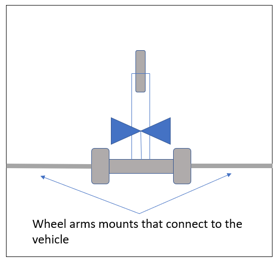
\includegraphics{images/part10/wheelmounts.png}
    \caption{Wheel arm mounts experimental setup}
    \label{fig:wheelmounts}
\end{figure}

The wheel mount connections available in the wind tunnel allow the load cells to be attached to the side of the vehicle. This method offers a single degree of measurement for the test, measuring the drag/thrust of the vehicle. The stabilization of the load cells will provide enough restoring moment on the vehicle, meaning the vehicle will remain 
straight throughout the test. This increased the safety of the experiment and reduced the chances of causing damage to the vehicle or wind tunnel. With this method the force were measured on both sides of the vehicle, meaning the measurements were split. The voltage changes measured through the Wheatstone bridge circuits were therefore divided by two, introducing the need to have a high enough minimum resolution.


\begin{figure}[!htbp]
    \centering
    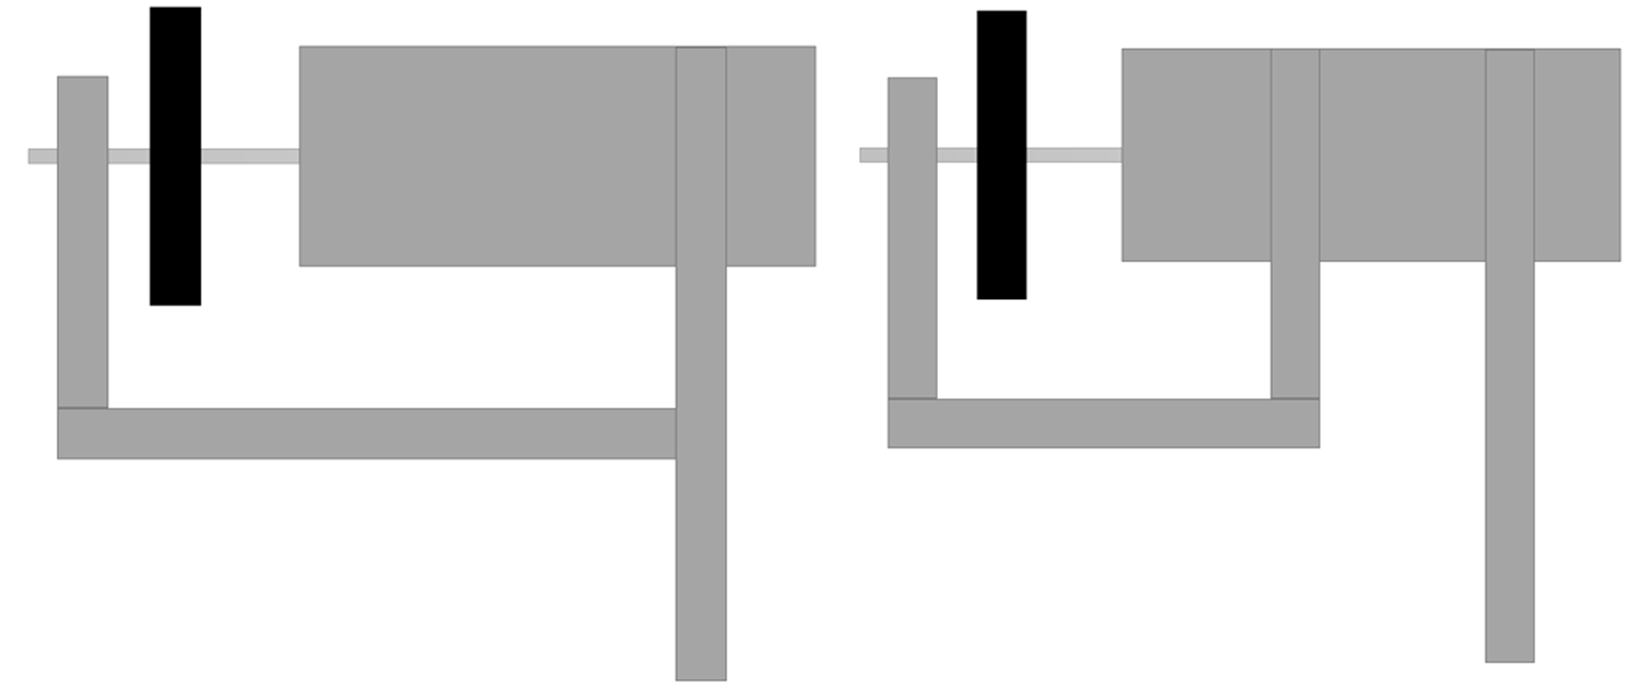
\includegraphics{images/part10/mountstruct.png}
    \caption{Structural extension possibilities. Option (1) on the left and option (2) on the right}
    \label{fig:mountstruct}
\end{figure}

\subsection{Two-wheel arm setup mounting}

Once the horizontal stabilisers were designed to be two straight bars going towards the front wheel, the focus turned to ensure that the model could be connected to the wheel arms of the wind tunnel. The issue faced was that there were no stable connections for the load cells to screw into. It was therefore required to design additional load cell connections for the wheel arms that would not affect the vehicle.

The closest part of the vehicle to the load cells would have been the axle rod of the back wheels. This component spins at the same RPM as the propeller and therefore would not be able to be directly connected to for a stable connection for the load cell. To overcome this issue, pillow bearings for the axle rod were used to allow components to be connected to the vehicle. 

The pillow bearings used allowed for the aluminium profile to be drilled and connected with screws which was beneficial for the vehicle as it maintained the modularity of the structure. To increase the stability of the load cell connection it was required to secure the bar to another section on the vehicle. This meant that the load cell would not oscillate significantly when the vehicle was rolling on the rolling road.

After consideration the two main locations for connecting the bar were the front wheel structural connections (1) and the metal plate on the other side of the wheel (2):


\begin{table}[H]
\caption{Advantages and disadvantages for the location of the wheel arm connection}
\label{tab:wheelArmConnection}
\centering
\begin{tabular}{|
>{\columncolor[HTML]{\CellColor}}l |p{7cm}|p{7cm}|}
\hline
\textbf{Option} & \cellcolor[HTML]{\CellColor}\textbf{Advantages}                                                           & \cellcolor[HTML]{\CellColor}\textbf{Disadvantages}                                                                   \\ \hline
\textbf{1}      & Stronger connection, less material used, added structural components to   the horizontal stabilisers. & Deformation with the vehicle oscillation possible, more pressure on   ensuring that the measurements are connect \\ \hline
\textbf{2}      & Mitigated deformation, as the bars are connected to two parts that are   mounted on the axle          & Increased material use, more cuts of the bar to manufacture                                                      \\ \hline
\end{tabular}
\end{table}

It was decided that it was better to connect the load cell mounts directly to the horizontal stabilisers of the vehicle to ensure that the structure would have the largest stiffness possible.

\subsection{Calibration}

Before the wind tunnel tests, an assessment of the load cell resolution was necessary to ensure force variations of the scale of those anticipated would be picked up by the sensors.  To analyse the performance of the cells, calibration of a spare set of load cells was conducted. 

To assess the resolution of the load cells, more focus was put on the lower weight ranges, taking note of the jump in force measurement of the data acquisition. The forces that were expected from the vehicle, especially at equilibrium points were expected to be low in comparison to scaled race car models operating at speeds of 40 m/s, which are more commonly tested using this setup. Therefore, small changes in drag/thrust could be key to properly discovering the behaviour of the vehicle in the wind tunnel. 

By completing five different calibrations it was found that the smallest change in force measurement for the load cells used for the wind tunnel was 0.06 N. As the prototype was expected to generate significantly more thrust/drag it was concluded that the resolution of the load cells was high enough.

\subsection{Wheels on or wheels off}

For the wind tunnel model, a decision had to be made on what type of testing would be beneficial for the model. The wheel-on model takes a vehicle as it is and puts it in a wind tunnel, whereas the wheels-off setup consists of the main body being detached from the wheels.

For the wheels-off testing, the model would require an active suspension system on each wheel. They would each be fitted with a motor that would drive the wheel and simulate the movement via push and pull rods. In general, the wheels-off system facilitates investigating the vehicle behaviour, focusing more on the vehicle interaction with the wind. Nevertheless, the wheels-on model required a shorter setup time, reducing the use of technician time for extra components. The added benefits of reducing the complexity of the vehicle were that it ensured that the wind tunnel tests could be conducted in the most efficient way possible. The wheels-off model would also require a more robust suspension and a more intricate drivetrain, further demonstrating the benefits of the wheels-on testing.

\begin{figure}
    \centering
    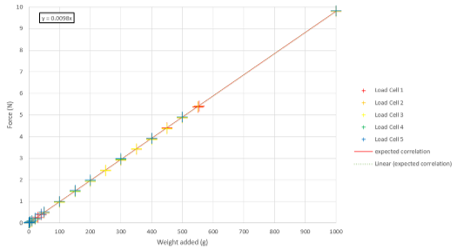
\includegraphics{images/part10/loadcellcal.png}
    \caption{Load cell calibration plot}
    \label{fig:loadcellcalib}
\end{figure}

\subsection{Data acquisition and processing}

A program called “Wheel Interface” collects and displays the readings from the load cells in real time. This data is inputted into a second program called “InCar”. The latter handles all the measurements as well as the speed of the wind in the wind tunnel and the rolling ground, the temperature, and the pressure. It communicates directly with the wind tunnel operator’s computer, which enables us to script the acquisition of data according to the operational status of the wind tunnel.

Hence a typical script for the experiments would be the following: Firstly, check to see if the speed of the rolling road and the wind are at the values required for the test. When this is met, an alert is sent to the wind tunnel operator, and only when he responds to it can the rest of the script be executed. The wind tunnel operator checks to see if the speeds of the rolling ground and/or wind tunnel have stabilised to the required value then proceeds to answer the alert. The rest of the script then runs and acquires the data. Each “acquire” function averages the data over an acquire period set beforehand, then writes the result to the output file. This period has a minimum of 1 second. After a few iterations, it was found that a reliable way to collect the data was to have a short acquiring period of 1 or 2 seconds and have 15 to 30 “acquire” functions for one specific run. This is done to get as many details on the variance of the data as possible. After the acquisition is over, the rolling road and wind speed can be modified to the next required speeds and the process is looped. The output file from this program comes in the form of Microsoft Access database files. Comments are added via “InCar” to differentiate the runs.





\subsection{Vehicle drag numerical prediction methodology}

A steady state RANS CFD analysis in Ansys Fluent has been conducted for the vehicle. An unstructured mesh with one million cells was used. The Menter $k-\omega SST$ turbulence model was used with use of a wall function for the first cells from the wall. Here, as stated in the users manual \cite{usrguide}, the transport equation for the turbulence kinetic energy and $\omega$ , used to find the turbulence viscosity, takes the form:

\begin{equation}
\frac{\partial}{\partial t}(\rho k)+\frac{\partial}{\partial t}\left(\rho k u_{i}\right)=\frac{\partial}{\partial x_{j}}\left(\Gamma_{k} \frac{\partial k}{\partial x_{j}}\right)+\widetilde{G_{k}}-Y_{k}+S_{k}
\end{equation}

\begin{equation}
\frac{\partial}{\partial t}(\rho \omega)+\frac{\partial}{\partial t}\left(\rho \omega u_{i}\right)=\frac{\partial}{\partial x_{j}}\left(\Gamma_{\omega} \frac{\partial \omega}{\partial x_{j}}\right)+G_{\omega}-Y_{\omega}+S_{\omega}+D_{\omega}
\end{equation}

Where the terms G,Y,and S with their subscript letters represent the generation of turbulence kinetic energy due to mean velocity gradients, dissipation, and user defined source terms respectively. $\Gamma_k$,$\Gamma_\omega$ are the effective turbulence diffusivity terms, and $D_\omega$ is the cross-diffusion term used to determine the value of $F_1$, a blending parameter which blends the $k-\epsilon$ model into the $k-\omega$ model for the cells with a cell height that puts it into the log law region, which will be the case for the majority of the cells in this simulation. 

The above models are used to close the Reynolds stress terms in the Navier-Stokes equations:

\begin{equation}
\frac{\partial \rho}{\partial t}+\frac{\partial}{\partial x_{i}}\left(\rho u_{i}\right)=0
\end{equation}
\begin{equation}
\frac{\partial}{\partial t}\left(\rho u_{i}\right)+\frac{\partial}{\partial x_{i}}\left(\rho u_{i} u_{j}\right)=-\frac{\partial p}{\partial x_{i}}+\frac{\partial}{\partial x_{j}}\left(\mu\left(\frac{\partial u_{i}}{\partial x_{j}}+\frac{\partial u_{j}}{\partial x_{i}}-\frac{2}{3} \delta_{i j} \frac{\partial u_{i}}{\partial x_{i}}\right)\right)+\frac{\partial}{\partial x_{j}}\left(-\rho \overline{u_{l}^{\prime} u_{j}^{\prime}}\right)
\end{equation}

Using the semi-implicit method for pressure linked equations-consistent (SIMPLEC) algorithm, normalised residuals of $10^{-4}$ were achieved for each simulation.

A 10m radius 10m long C-type domain with 4604517 cells was used with the wheels in contact with the bottom wall. Because of symmetry properties, the domain was halved in the centre vertically with a symmetry boundary condition. The bottom wall was set as an inviscid wall with no shear stress to apply an impermeability condition as well as to eliminate boundary layer effects. The turbulent intensity and turbulent viscosity ratio was set to 5\% and 10 respectively at the inlet, suitable for unbounded flows, as stated in the user’s manual
 \cite{usrguide}.

An unstructured mesh without a boundary layer mesh (Figure \ref{fig:vehiclesidemesh}) was used with the majority of the cells located in the log law region of $30<Y+<300$ was used. Some areas including the rear side of the wheels where the flow velocity is low, the Y+ values were either low or in the buffer region, making the $k-\omega$ more suited than the $k-\epsilon$ with enhanced wall treatment due to $k-\omega$ model's switching nature.

\begin{figure}[!htbp]
    \centering
    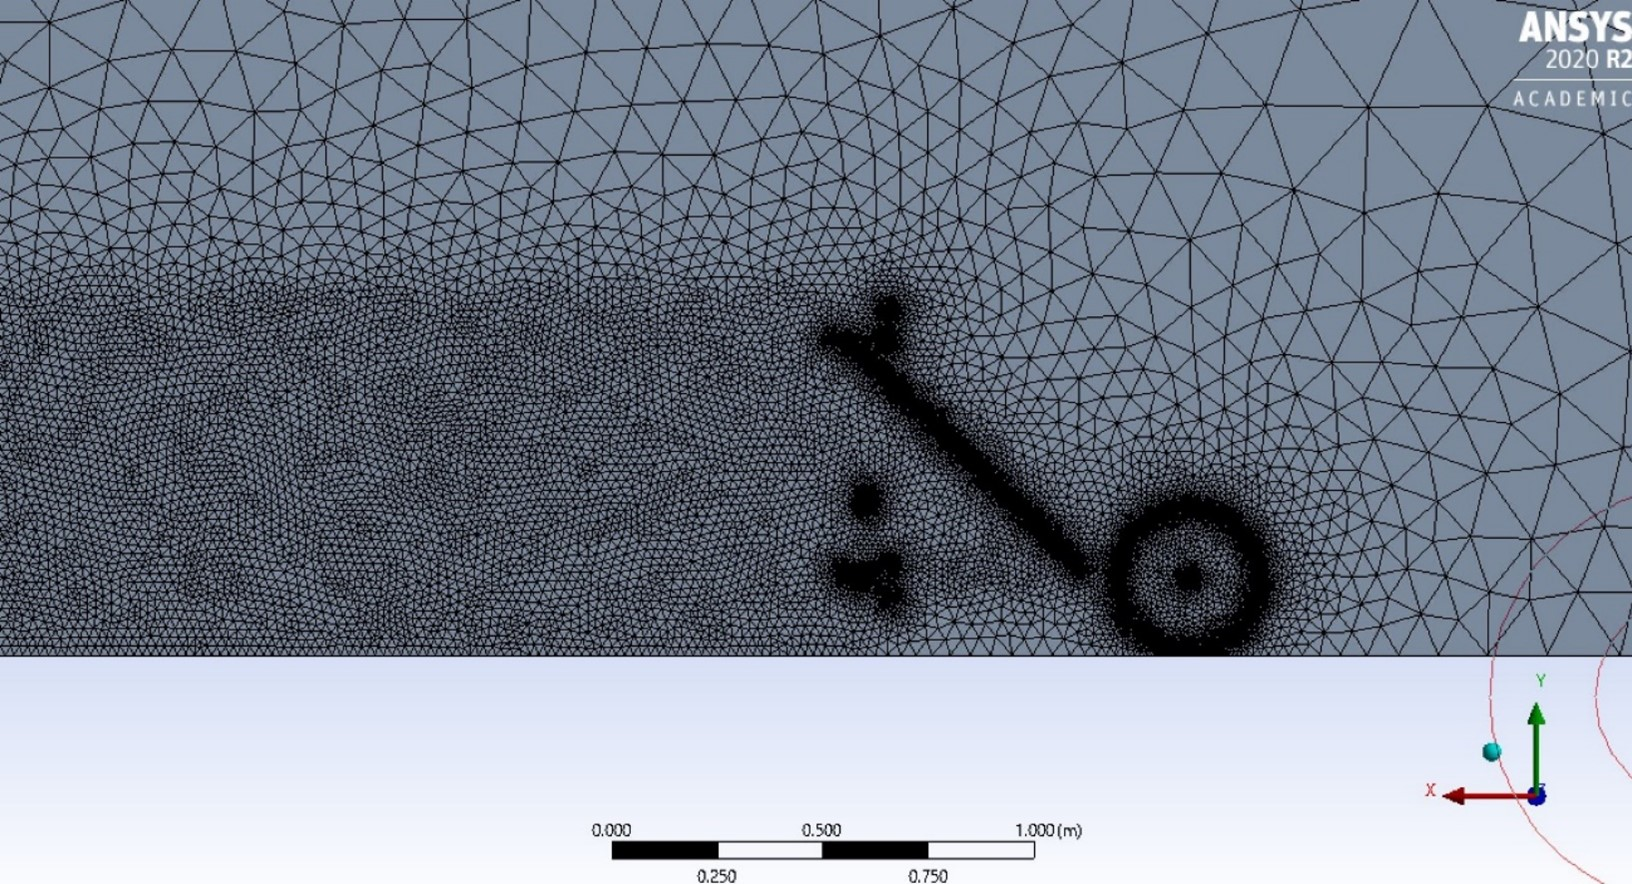
\includegraphics{images/part10.1/vehiclemesh.jpg}
    \caption{Side view of the vehicle mesh normal to the symmetry plane}
    \label{fig:vehiclesidemesh}
\end{figure}

A grid study was conducted on the vehicle model in the form of global and wake refinements.
Refinement of the wake from the axle position to the downstream end of the domain was first conducted (Figure \ref{fig:dragncells}). 


A study on the global sizing of the mesh where the maximum element size decreased was made. The element sizes in the region near the vehicle was kept unchanged.

It can be observed that a very coarse setting for the wake refinement causes an unexpected decrease in the drag. It is thought that at this point the interpolation between the cells is causing an error in flow variables in a different way to the more fine variants of the mesh. Further increasing the mesh density to 4 million cells causes an exponential decrease in the drag prediction which approaches the experimental value.



\subsection{Propeller performance numerical prediction methodology}

A URANS study on the performance of the propeller using computational fluid dynamics (CFD) in Ansys Fluent was conducted. Using these results, the thrust and torque applied to the shaft can be found and used to predict the drag imposed on the vehicle. The study gives further insight as to what parameters in the design alter the performance. For this study, the zero wind speed case was investigated. A case that closely matches the configuration of the fine or otherwise called the minimum pitch case, and a hypothetical extreme coarse or high pitch case has been tested. The coarse pitch case has been tested as an extreme case as a demonstration and is therefore not a representation of the experimental high pitch case.  

The propeller model was put into a rotating domain of radius 0.36m and thickness 0.4m and rotated at various rotation rates, with the inlet velocity kept at zero to simulate experimental conditions. A rectangular static domain with dimensions 3x3x5m was used to more closely simulate conditions in the wind tunnel while keeping sufficient distance from the inlet. The sidewalls of the domain were set as walls with a specified shear stress of zero to enforce an impermiability condition. In a study of the grid, it was found that a finer mesh increases the thrust and decreases the moment applied to the propeller. In response to a decrease in size from 0.04m to 0.01m size of cells, the thrust was found to increase by 6\%. To reach a sufficiently low sensitivity in mesh density, a further study with a comparison of more dense meshes would be required, but the current study gives a good understanding in a quantitative aspect of the performance of the propeller. The semi-implicit method for pressure linked equations-consistent (SIMPLEC) was used to solve the Navier-Stokes equations.

 
\begin{figure}[!htbp]
    \centering
    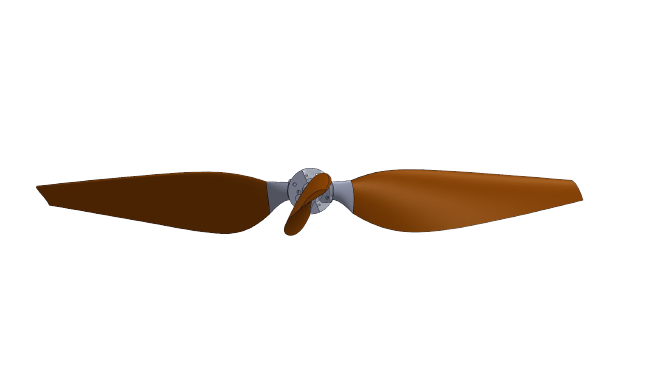
\includegraphics{images/part10.1/highpitch-removebg-preview.png}
    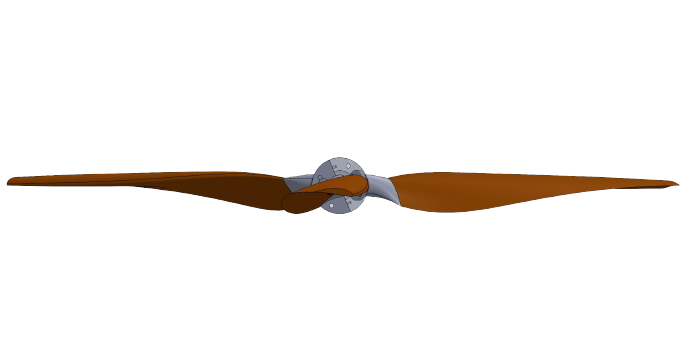
\includegraphics{images/part10.1/lowpitch-removebg-preview.png}
    \caption{Side view of the propeller in a high-pitch configuration (top) and low-pitch configuration (bottom)}
    \label{fig:pitches}
\end{figure}

\begin{figure}[!htbp]
    \centering
    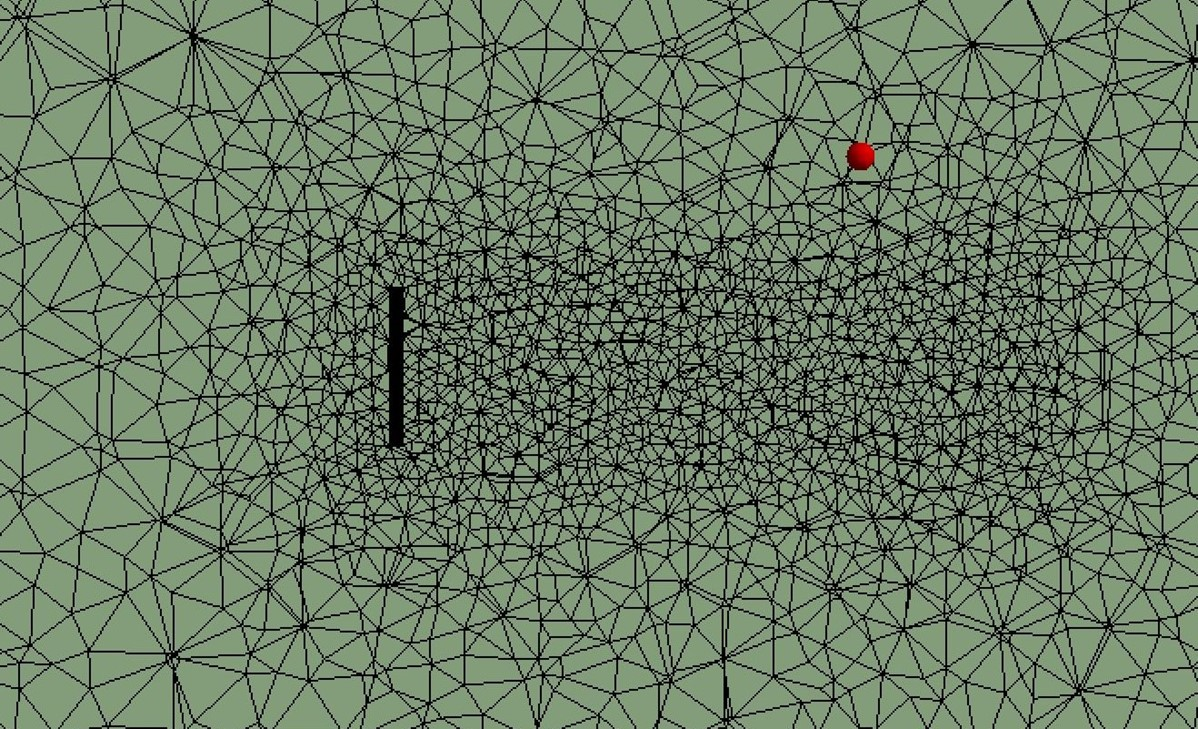
\includegraphics{images/part10.1/propdomain.jpg}
    \caption{Section view of the grid of the static domain of the propeller. The black rectangle is the rotating domain containing the propeller.}
    \label{fig:propellersidemesh}
\end{figure}

\begin{figure}[!htbp]
    \centering
    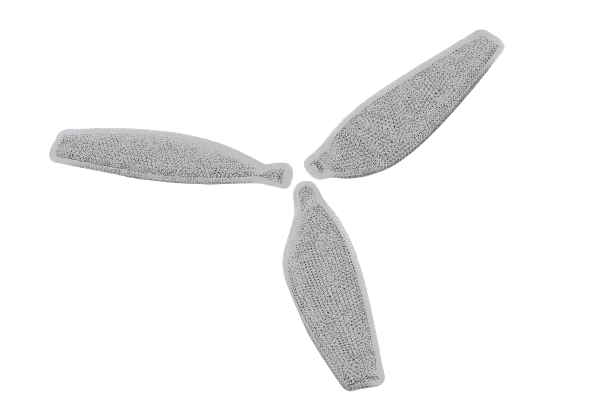
\includegraphics{images/part10.1/propmesh-removebg-preview.png}
    \caption{Mesh of the propeller (fine pitch setting)}
    \label{fig:propellermesh}
\end{figure}

\begin{figure}[!htbp]
    \centering
    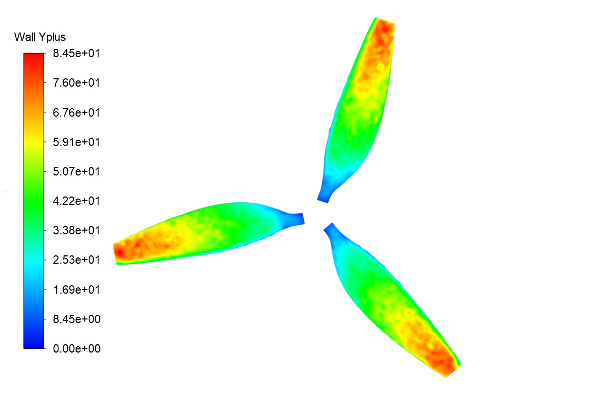
\includegraphics{images/part10.1/Yplus_refined_mesh-removebg-preview_integrated.png}
    \caption{$Y^+$ contour plot at the surface of the propeller mesh}
    \label{fig:propelleryplus}
\end{figure}

An unstructured mesh without a structured boundary layer mesh was used, and sizing of the cells within the rotating domain varied to achieve the desired $Y^+$ range of 30 - 300 for 63\% of the surface from the tip to the root. It was found a coarser mesh than this would decrease the accuracy due to not resolving curvature correctly, but a mesh too fine would cause the regions of high velocity of the propeller to be in the buffer region.
